\documentclass[11pt,a4paper]{report}

\usepackage{amsmath}
\usepackage{graphicx}
\usepackage{hyperref}

\graphicspath{{images/}}

\begin{document}

\title{Part C Project Notes}
\author{Catherine Vlasov}
\maketitle

%-----------------------
\tableofcontents


%-----------------------
\chapter{Task Documentation}

All timings mentioned here are approximate. The specific results can be found in Section \ref{sec:script-timings}.

\section{Image Curation}

\subsection{Initial Image Selection}
\label{subsec:initial-image-selection}

The first step was selecting which images to use for the experiments. Flickr released a massive database of millions of images and we will use those taken by one user, referred to as \texttt{actor00003}. There are $13,349$ images taken by this user and they are on the server under \texttt{/array/vlasov/actor00003}. The largest image size in this directory is $3072\times2304$ pixels and information about all the images is in a file called \texttt{metadata.txt} in the same directory.

I wrote a script called \texttt{initial\_curation.py} to do the initial image filtering. The script uses the metadata file to identify the images that are $3072\times2304$ pixels, makes all of these images grayscale, rotates the portrait ones to landscape, and places the resulting images in a new subdirectory called \texttt{size3072}. The script took around 10 minutes to run and 9539 grayscale, $3072\times2304$ pixel, landscape images were produced.


\subsection{Choosing Image Sizes}
\label{subsec:image-sizes}

The largest size is $3072\times2304$ since that is the largest size we have from \texttt{actor00003} and the smallest size was somewhat arbitrarily chosen to be $360\times240$. In the graphs with my experiment results, I will want the image sizes (specifically the total number of pixels) to be evenly distributed along the x-axis. In order to achieve this, I picked sizes such that the difference between the number of pixels in consecutive image sizes is roughly the same. I calculated this interval using:
\begin{equation*}
\frac{3072 \cdot 2304 - 320 \cdot 240}{9} \approx 777,899 \text{ pixels}
\end{equation*}

It is straightforward to compute the total number of pixels in the $n^{th}$ image size (where $320 \times 240$ is the $1^{st}$ size and $3072 \times 2304$ is the $10^{th}$ size):
\begin{equation*}
320 \cdot 240 + (n-1) \cdot 777,899
\end{equation*}

Given the desired number of pixels (call it $P$), we can find dimensions with a 4:3 ratio that produce approximately $P$ pixels. We do so by solving the following equation for $x$ and then computing $4x$ and $3x$ to get the dimensions:
\begin{equation*}
 P \approx 4x \cdot 3x = 12x^2
 \end{equation*}

The results of these computations are:
\begin{center}
\begin{tabular}{ c  c | c}
Width & Height & Total pixels \\ \hline
3072 & 2304 & 7,077,888 \\
2912 & 2184 & 6,359,808 \\
2720 & 2040 & 5,548,800 \\
2528 & 1896 & 4,793,088 \\
2304 & 1728 & 3,981,312 \\
2048 & 1536 & 3,145,728 \\
1792 & 1344 & 2,408,448 \\
1472 & 1104 & 1,625,088 \\
1056 & 792 & 836,352 \\
320 & 240 & 76,800 \\
\end{tabular}
\end{center}

\subsection{Cropping}
\label{subsec:cropping}


%-----------------------
\chapter{Meeting Notes}

\section{07/11/18}

\begin{itemize}

\item What I did:
  \begin{itemize}
  \item Created the file structure on the server.
    \begin{itemize}
    \item Each \texttt{actor00003/sizeXXXX/} directory only has one subdirectory called \texttt{cover} since we need to decide/calculate how many bits of payload to embed for each size.
    \end{itemize}

  \item Changed \texttt{initial\_curation.py} so that constants in the file are instead passed in as command-line arguments.
    \begin{itemize}
    \item Reran it and it was almost twice as fast (11 vs 19 minutes).
    \end{itemize}

  \item Finished \texttt{compute\_probabilities.py}. It finds a $\lambda$ such that:
    \begin{equation*}
    \sum\limits_{i=1}^N H_2(\pi_i) \in [m, m+1)\text{, where $m$ is the payload size to simulate}
    \end{equation*}

  \item Wrote \texttt{crop.py} and ran it for the other nine image sizes.
    \begin{itemize}
    \item It crops $8\times8$ blocks evenly from the top/bottom and right/left.
    \item The process is documented in Section \ref{subsec:cropping}.
    \end{itemize}
  \end{itemize}

\end{itemize}

\section{31/10/18}

\begin{itemize}

\item What I did:
  \begin{itemize}
  \item Put together this document
  \item Organized all documents and scripts in my (private) GitHub repository
  \item Fixed \texttt{initial\_curation.py} (the problem is documented in Section \ref{sec:lessons-learned}) and I successfully ran it on the server
    \begin{itemize}
    \item Original images: \texttt{/array/vlasov/actor00003/original}
    \item All $3072\times2304$, grayscale, landscape images are in a new directory \texttt{/array/vlasov/actor00003/size3072}
    \end{itemize}
  \item Learned how to use \texttt{pyplot}, plotted $H_2$ as an exercise
  \item Computed the image sizes we'll use (the process and results are described in Section \ref{subsec:image-sizes})
    \begin{itemize}
    \item The method discussed on 24/10/18 doesn't work. It does produce equally sized intervals (in terms of the difference in the total number of pixels between consecutive sizes), but only between $320\times240$ and the ninth-largest size since this interval is only around $70,000$. The ninth-largest size would be $960\times720$, which is clearly much smaller than $3072\times2304$.
    \item In order to get sizes linearly distributed in terms of the total number of pixels, the interval needs to be closer to $700,000$ pixels.
    \end{itemize}
  \item Started working on \texttt{compute\_probabilities.py}
  \end{itemize}

\item \textit{Is the value of $\lambda$ bounded? How should the binary search (in the context of PLS) work?}
  \begin{itemize}
  \item $\lambda = 0$ corresponds to maximum entropy (aka. maximum payload) because then $\pi_i = \frac{1}{1+e^{\lambda c_i}} = \frac{1}{2}$

  \item As $\lambda \rightarrow \infty$, $\pi_i \rightarrow 0$

  \item The order of magnitude of $\lambda$ depends on the order of magnitude of the costs.

  \item The binary search will have two stages:
    \begin{enumerate}
    \item Exponential search to find an upper bound on $\lambda$. This will involve trying exponentially large values such as $0, 1, 10, 100, ...$ until a value is found such that $\sum\limits_{i=1}^N H_2(\pi_i) < M$
    \item Suppose the first value where this inequality holds is $\lambda = 10^n$. We now do a binary search for $\lambda$ with a lower bound of $10^{n-1}$ and an upper bound of $10^n$ and we want to find a value such that $\sum\limits_{i=1}^N H_2(\pi_i) \in [m, m+1)$, where $m$ is the number of payload bits.
    \end{enumerate}
  \end{itemize}
  
\item In Dr. Ker's paper ``On the Relationship Between Embedding Costs and Steganographic Capacity'' from June 2018, he writes about how if the detector knows the costs $c_1, c_2, ... c_N$, then the objective that should be minimized is $\sum\limits_{i=1}^N c_i \pi_i^2$, which is the same as the objective in PLS except with the $\pi_i$ terms squared.
  \begin{itemize}
  \item This is a possible project extension.

  \item The tricky part is computing the probabilities since the optimal solution is no longer $\pi_i = \frac{1}{1+e^{\lambda c_i}}$. Instead, it's $\frac{\pi_i}{H2'(\pi_i)} = \lambda c_i$.

  \item The probabilities can be computed by running Newton-Raphson several times (Dr. Ker did it 8 times)

  \item I don't need to tackle this now, but it's worth keeping in mind.
  \end{itemize}

\item When I use Dr. Ker's J-UNIWARD hack, I need to make sure that I work out the order in which the costs are written to the file.
  \begin{itemize}
  \item It's hard to tell just by looking at the costs whether or not they're in the right order. If I'm wrong, I'll probably find out since the embedding will be very detectable.
  \item It's very likely that the $8\times8$ blocks are analyzed from left to right, top to bottom. However, within each block the costs could be left to right, top to bottom \textbf{or} in the zigzag order used to store the quantized coefficients. I need to check this.
  \end{itemize}

\item Once I compute the probabilities, it might be a good idea to use Python's \texttt{random.seed(..)} method (with the image number as the seed) in order to do the embedding. It can be used to determine whether or not to change each coefficient and so I'll always get the same embedding with the same cover, modulo rounding.

\item Dr. Ker has a faster version of JRM for feature extraction.

\item Tips:
  \begin{itemize}
  \item After embedding, open the stego image to make sure nothing got messed up (e.g. due to the order of the costs or coefficients).

  \item It would be a good idea to write some scripts to check things like:
    \begin{itemize}
    \item The number of coefficients that differ between the cover and stego images is $\approx \sum\limits_{i=1}^N \pi_i$
    \item Coefficients that differ between the cover and stego images only differ by $\pm1$
    \end{itemize}

  \item Test things out on small images (e.g. $64\times64$) to save time in case there are bugs.
  \end{itemize}

\end{itemize}


\section{24/10/18}

\begin{itemize}

\item What I did:
  \begin{itemize}
  \item Read Chapter 3 of the Advanced Security notes on steganography
  \item Wrote a script (\texttt{initial\_curation.py}) to find all the largest images in the \texttt{actor00003} directory and then make them all grayscale and landscape (described in Section \ref{subsec:initial-image-selection})
    \begin{itemize}
    \item Wasn't quite working due to ``\texttt{Empty input file}'' error when performing multiple \texttt{jpegtran} operations
    \end{itemize}
  \end{itemize}

\item Action plan:
  \begin{enumerate}

  \item Calculate image sizes
    \begin{itemize}
    \item Preserve the 4:3 aspect ratio, not because we have to but because we can and it means we can keep things as similar as possible

    \item The largest image size we'll use is $3072\times2304$ since that's the size of the largest \texttt{actor00003} images.

    \item The smallest size will be $320\times240$ since that's a relatively common image size (and it has a 4:3 aspect ratio)

    \item The short-edge dimensions will be computed by hand by calculating $240x$ (where $x=\sqrt{1}, \sqrt{2},...,\sqrt{10}$) and then rounding to the nearest multiple of 24. Then the long-edge dimensions are calculated such that the 4:3 ratio is maintained.
    \end{itemize}

  \item Create the directory structure on the server in \texttt{/array/vlasov/}
    \begin{itemize}
    \item Keep a copy of all the original images in \texttt{actor00003/original}

    \item Create one directory per image size, called \texttt{size3072} (for instance)

    \item For each size, create two subdirectories:
      \begin{enumerate}
      \item One for the unaltered images, called \texttt{cover}
      \item One per number of payload bits, called \texttt{stego-1234bits}
      \end{enumerate}

    \item Each \texttt{cover} subdirectory will have three files per cover image:
      \begin{enumerate}
      \item \texttt{image12345.jpg}: the unaltered image
      \item \texttt{image12345.costs}: the costs computed by J-UNIWARD
      \item \texttt{image12345.fea}: the features computed by JRM
      \end{enumerate}

    \item Each \texttt{stego-1234bits} subdirectory will have one file per stego image:
      \begin{enumerate}
      \item \texttt{image12345.jpg}: the stego image, which is the cover image \texttt{sizeXXXX/cover/image12345.jpg} with a 1234-bit message embedded in it
      \end{enumerate}
    \end{itemize}

  \item Crop the $3072\times2304$ cover images to the sizes calculated in task 1. Do this by cropping $8\times8$ pixel blocks evenly from the top/bottom and right/left.

  \item Generate the costs (using Dr. Ker's slighty modified J-UNIWARD code) and features (using JRM) for all the cover images of all the different sizes.
  \begin{itemize}
  \item JRM produces 22510 real numbers (the features)
  \item Up to me how to store them, but ASCII is probably the most portable
  \end{itemize}

  \item Use J-UNIWARD to embed 0.4 bits per non-zero AC coefficient in some of the covers.

  \item Write a function that takes the number of payload bits as input and computes the probabilities with which each coefficient changes during (binary) embedding.
    \begin{itemize}
    \item Goal: given the costs $c_1, c_2, ... c_N$ (where N is the total number of coefficients) of changing each coefficient (by adding or subtracting one), compute the probabilities $\pi_1, \pi_2, ..., \pi_N$ of making each of these changes

    \item Size of the payload: $\sum\limits_{i=1}^N H_2(\pi_i)$
      \begin{itemize}
      \item $H_2$ is the ``entropy'' and is defined as:
        \begin{equation*}
        H_2(x) = -x \cdot \log_2 x - (1-x) \cdot \log_2 (1-x)
        \end{equation*}

      \item Graph of $H_2$:
        \begin{center}
          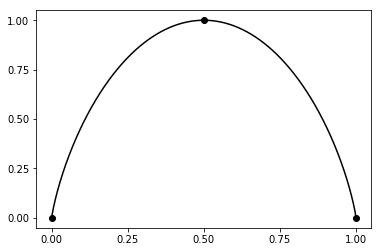
\includegraphics[width=0.7\linewidth]{h2_plot.png}
        \end{center}
      \end{itemize}

    \item Average total cost: $\sum\limits_{i=1}^N c_i \pi_i$

    \item Two (equivalent) optimization problems for computing the payload size:
      \begin{enumerate}
      \item Distortion-limited sender (DLS)
        \begin{equation*}
        \text{Maximize } \sum\limits_{i=1}^N H_2(\pi_i) \text{ such that } \sum\limits_{i=1}^N c_i \pi_i \leq C
        \end{equation*}

      \item Payload-limited sender (PLS)
        \begin{equation*}
        \text{Minimize } \sum\limits_{i=1}^N c_i \pi_i \text{ such that } \sum\limits_{i=1}^N H_2(\pi_i) \geq M
        \end{equation*}
      \end{enumerate}

    \item For some fixed $\lambda$, we can compute the probabilities:
      \begin{equation*}
      \pi_i = \frac{1}{1+e^{\lambda c_i}}
      \end{equation*}

    \item We'll use PLS, where M is the payload size.
      \begin{itemize}
      \item The optimal solution is when $\sum\limits_{i=1}^N H_2(\pi_i) = M$
      \item $\sum\limits_{i=1}^N H_2(\pi_i)$ is actually monotonically decreasing, so we can find a value of $\lambda$ such that $\sum\limits_{i=1}^N H_2(\pi_i) = M$ for any M we choose. Then, we can compute the probabilities $\pi_1, \pi_2, ..., \pi_N$ using this value of $\lambda$.
      \item The end goal is to do the embedding ourselves by modifying each coefficient with these probabilities.
      \end{itemize}
    \end{itemize}

  \end{enumerate}

\item \textit{Is 80 a standard JPEG quality factor (QF)?} In the massive image database released by Flickr, the most common QFs were 100, the QF used by iPhones, and 80. So, we're using 80 because that gives us a greater selection of images.

\end{itemize}


\section{17/10/18}

\begin{itemize}

\item What I did:
  \begin{itemize}
  \item Read Chapters 1 and 2 of the Advanced Security notes on steganography
  \item Read the 2008 paper ``The Square Root Law of Steganographic Capacity''
  \end{itemize}

\item Discussed questions I had about Chapter 1 (Steganography) and Chapter 2 (Steganalysis) of the Advanced Security notes and about the 2008 paper.
  \begin{itemize}

  \item \textit{What is downsampling?} Shrinking

  \item \textit{When you take a pictures on your phone, what happens?} Captures raw image, immediately compresses it as a JPEG, and discards the raw image

  \item \textit{What determines a cover's ``source''?} Primarily the camera. The camera's ISO setting, in particular, is very important. The subject of the photos don't make much of a difference.

  \item \textit{In JPEG compression, don't you lose some information when dividing the image into $8\times8$ pixel blocks?} No, the DCT is linear (i.e. 1-to-1 mapping from $8\times8$ blocks to coefficients)

  \item \textit{Is a JPEG decompressed every time you view it on a computer?} Yes

  \item \textit{When LSBR is used on RGB images, which bit(s) are changed?} Good question - it depends, but usually the LSBs of all three components (in sync)

  \end{itemize}

\item After embedding a payload, the original cover is destroyed. Otherwise, two nearly identical images would be floating around and Alice could easily be outed if someone got their hands on both versions.

\end{itemize}


\section{03/10/18}

\begin{itemize}

\item What I did: N/A

\item Discussed software to be used for embedding (J-UNIWARD), feature extraction (JRM), and detection (ensemble of linear classifiers)
  \begin{itemize}
  \item All the software is \href{http://dde.binghamton.edu/download/stego_algorithms/}{here}
  \end{itemize}

\item Server's IP: 163.1.88.150

\item Amounts of payload to embed: $O(1)$, $O(\sqrt{n})$, $O(\sqrt{n} \log n)$, $O(n)$

\item $m \sim \frac{\sqrt{DC}}{2} \log \frac{C}{D}$

\item TIME EVERYTHING

\item I will test new embedding and new detecting methods and I could also try old embedding and new detecting methods

\item Total amount of space needed (assuming around 10,000 images are used):
  \begin{itemize}
  \item Images: $2MB \times 10000 \times 9 \approx 180GB$
  \item Costs: $8B \times 5M \times 10000 \approx 400 GB$
  \item Features: $170KB \times 10000 \times 9 \approx 17GB$
  \end{itemize}

\end{itemize}


%-----------------------
\chapter{Notes to Self}

\section{Useful Commands}

\begin{itemize}

\item Run a command in the background so that you can keep using the terminal or close it
  \begin{itemize}
  \item \texttt{nohup python script.py \&> script\_output.out \&}
  \end{itemize}

\item Check on processes that are running
  \begin{itemize}
  \item \texttt{ps aux | grep vlasov}
  \end{itemize}

\end{itemize}


\section{Script Timings}
\label{sec:script-timings}

\begin{itemize}

\item \texttt{initial\_curation.py} (before I changed constants to command-line arguments)
  \begin{itemize}
  \item $1131.18478608s \approx 18m51s$ (30/10/18)
  \end{itemize}

\item \texttt{initial\_curation.py --from-dir original/} \\ \texttt{--to-dir size3072/cover/}
  \begin{itemize}
  \item $655.185225964s \approx 10m55s$ (01/11/18)
  \end{itemize}

\item \texttt{crop.py --from-dir size3072/cover --to-dir sizeW/cover/} \\
         \texttt{ --width W --height H}, where:
  \begin{center}
  \begin{tabular}{ c c | c c | c }
  W & H & Seconds & Approx. Time & Date\\ \hline
  2912 & 2184 & 689.414359808 & 11m29s & 01/11/18 \\
  2720 & 2040 & 662.552460909 & 11m02s & 01/11/18 \\
  2528 & 1896 & 662.54279089 & 11m02s & 01/11/18 \\
  2304 & 1728 & 632.872202158 & 10m32s & 01/11/18 \\
  2048 & 1536 & 605.926501989 & 10m05s & 01/11/18 \\
  1792 & 1344 & 555.097690105 & 9m15s & 01/11/18 \\
  1472 & 1104 & 511.460752964 & 8m31s & 01/11/18 \\
  1056 & 792 & 438.49830699 & 7m18s & 01/11/18 \\
  320 & 240 & 359.436480045 & 5m59s & 01/11/18 \\
  \end{tabular}
  \end{center}

\end{itemize}

\section{Lessons Learned}
\label{sec:lessons-learned}

\begin{itemize}

\item The input and output file to \texttt{jpegtran} can't be the same, otherwise you get an ``\texttt{Empty input file}'' error.

\item If it looks like directories on the server have disappeared, turn off f.lux or change the colour settings in \texttt{.bashrc}.

\end{itemize}

\end{document}